%        File: presentation.tex
%     Created: Tue Apr 12 03:00 PM 2016 E
% Last Change: Tue Apr 12 03:00 PM 2016 E
%

\documentclass{beamer}
\usetheme{Frankfurt}
\usepackage{common}
%\usepackage{lmodern}% http://ctan.org/pkg/lm
%\usepackage{mathtools}
%\usepackage{amsmath}
%\usepackage{amssymb}
%\usepackage{stmaryrd}
%\usepackage{adjustbox}
%\usepackage{subfigure}
%\usepackage{graphicx}

  \title{Aerothermodynamic Design Sensitivities for a Reacting Gas Flow Solver
  on an Unstructured Mesh Using a Discrete Adjoint Formulation}

  \author{ Kyle B. Thompson }
\begin{document}
\begin{frame}
  \titlepage
\end{frame}
\begin{frame}
  \frametitle{Outline}
  \tableofcontents
\end{frame}
\section{Introduction}
\stepcounter{subsection}
\begin{frame}
  \frametitle{Introduction and Motivation}
  \begin{itemize}
    \item Exploring design space using high-fidelity CFD is challenging
    \item zero-order methods (sampling) are prohibitively expensive
    \item Need to be intelligent about techniques for evaluating sensitivity to
      design parameters
    \item Gradient-based optimization much more efficient than sampling, but
      requires calculating sensitivity derivatives
  \end{itemize}
\end{frame}
\begin{frame}
  \frametitle{Introduction and Motivation}
  \begin{itemize}
    \item How to compute sensitivity of design variables?
    \item Direct differentiation approach
      \begin{itemize}
        \item Navier-Stokes equations can be directly differentiated to yield
          sensitivity derivatives necessary for gradient-based optimization
        \item Requires a minimum of one flow solution for each design variable
          sensitivity
        \item Prohibitively expensive for large number of design parameters
      \end{itemize}
  \item Adjoint approach
    \begin{itemize}
      \item Solve adjoint equations in addition to Navier Stokes flow equations to
        obtain sensitivity derivatives
      \item One flow and adjoint solution needed for each cost function,
        regardless of number of design variables
      \item Considerably more efficient than direct differentiation approach for
        large number of design parameters
    \end{itemize}
  \end{itemize}
\end{frame}
\begin{frame}
  \frametitle{Introduction and Motivation}
  \begin{itemize}
    \item Adjoint-based design optimization has recieved considerable attention
      in compressible, perfect gas CFD solvers, but very little in reacting flow
      solvers
    \item Difficulty of adjoint approach lies in implementating exact
      linearizations for 2nd-order flux construction scheme
    \item Particularly difficult for reacting flows, due to 
      \begin{itemize}
        \item complexity of linearizing the additional equations for
          multi-species chemical kinetics
        \item Serious memory and computational cost concerns
      \end{itemize}
  \end{itemize}
\end{frame}
\begin{frame}
  \frametitle{Introduction and Motivation}
  \begin{itemize}
    \item Reacting gas simulations require solving a large number of conservation
      equations
    \item Memory concerns
    \begin{itemize}
        \item Size of Jacobians scales quadratically with number species in gas mixture
        \item Solving system of equations in a tightly-coupled fashion can be
          limited by memory constraints
    \end{itemize}
    \item Cost concerns
    \begin{itemize}
      \item Cost of solving the linear system scales quadratically with number
      of species in gas mixture
    \end{itemize}
    \item Efficiently solving adjoint problem is a primary motivator
      \begin{itemize}
        \item Solving adjoint system particularly costly if linear solver is
          slow
        \item Can be necessary to store jacobian twice $\to$ large memory
          overhead
      \end{itemize}
  \end{itemize}
\end{frame}
\begin{frame}
  \frametitle{Introduction and Motivation}
  \begin{itemize}
    \item Loosely-coupled solvers have become popular in the combustion
      community.
      \begin{itemize}
        \item Decouple species conservation equations from meanflow equations,
          and solve two smaller systems
         \[
           \underset{(4+ns) \times (4+ns)}
           {\begin{pmatrix}
             \boxempty & \boxempty & \dots  & \boxempty \\
             \boxempty & \boxempty & \dots  & \vdots \\
             \vdots    & \vdots    & \ddots & \vdots \\
             \boxempty & \dots     & \dots  & \boxempty
           \end{pmatrix}}
           \to
           \underset{5 \times 5}
           {\begin{pmatrix}
             \boxempty & \dots  & \boxempty \\
             \vdots    & \ddots & \vdots \\
             \boxempty & \dots  & \boxempty
           \end{pmatrix}}
           \text{and}
           \underset{ns \times ns}
           {\begin{pmatrix}
             \boxempty  & \boxbslash & \dots  & \boxbslash \\
             \boxbslash & \boxempty  & \dots  & \vdots \\
             \vdots     & \vdots     & \ddots & \vdots \\
             \boxbslash & \dots      & \dots  & \boxempty
           \end{pmatrix}}
         \]
    \end{itemize}
    \item Beneficial for adjoint formulation
    \begin{itemize}
      \item Two smaller systems are considerably easier to linearize
      \item Storing jacobian for adjoint solve becomes practical
    \end{itemize}
      \item Candler, et al. originally derived this for Steger-Warming scheme, this
        work extends to Roe FDS scheme
      \begin{itemize}
        \item Candler, G. V., Subbareddy, P. K., and Nompelis, I. ``Decoupled
          Implicit Method for Aerothermodynamics and Reacting Flows.'' \textit{AIAA
          Journal}, Vol. 51, no. 5, pp. 1245-1254.
      \end{itemize}
  \end{itemize}
\end{frame}
\section{Flow Solver}

\subsection{Fully-Coupled Method}
\stepcounter{subsection}
\begin{frame}
  \frametitle{Fully-Coupled Point Implicit Method}
  \begin{itemize}
    \item All work presented is for inviscid flows in chemical non-equilibrium,
      using a one-temperature model, but is extendable to viscous flows.
    \item Beginning with the semi-discrete form
    \begin{equation*}
    	\label{inv_flux_fv}
    	\frac{\partial \mU}{\partial t}
    	 + \frac{1}{V}\sum\limits_{f}(\vF\cdot\ms)^f = \mw
    \end{equation*}
    \begin{equation*}
    	\begin{matrix}
    	\mU=\begin{pmatrix}
       		\rho_1\\
    		\vdots \\
    		\rho_{ns} \\
    		\rho u \\
    		\rho v \\
    		\rho w \\
    		\rho E \\
    	\end{pmatrix},      &
     	\mathbf{F \cdot S} = \begin{pmatrix}
    		\rho_1  \overline{U} \\
    		\vdots \\
    		\rho_{ns} \overline{U} \\
    		\rho u \overline{U} + p s_x\\
    		\rho u \overline{U} + p s_y\\
    		\rho u \overline{U} + p s_z\\
    		(\rho E + p) \overline{U} \\
    	\end{pmatrix}S,    &
     	\mw = \begin{pmatrix}
        \dot\rho_1\\
    		\vdots \\
    		\dot\rho_{ns} \\
        0 \\
        0 \\
        0 \\
        0
      \end{pmatrix}

  	\end{matrix}
  \end{equation*}

  \end{itemize}
\end{frame}
\begin{frame}
  \frametitle{Fully-Coupled Point Implicit Method}
  \begin{itemize}
  \item Using the Roe FDS scheme to compute the inviscid flux at the face,
    $\vF^f$, and linearizing the system results in
  \begin{multline*}
  	\frac{\mathbf{\delta U}^n}{\Delta t}
    +\frac{1}{V}\sum\limits_{f}(\frac{\partial \vF^f}
    {\partial \ul}\delta\mU^L
  	+\frac{\partial \vF^f}{\partial \ur}\delta\mU^R)^n \ms^f
  	- \frac{\partial \mw}{\partial \mU}\delta\mU^n \\
  	= -\frac{1}{V}\sum\limits_{f}(\vF^f\cdot\ms^f)^n + \mw^n
  \end {multline*}
  \item Which can be thought of more simply as
  \[
    \ma\vu = \vb
  \]
  \begin{align*}
    \ma &\to
    \begin{array}{c}
      (4+ns) \times (4+ns) \\
      \text{Jacobian Block}
    \end{array} \\
    \vb &\to
    \begin{array}{c}
      (4+ns) \times 1 \\
      \text{Residual}
    \end{array}
  \end{align*}
  \end{itemize}
\end{frame}
\begin{frame}
  \frametitle{Fully-Coupled Point Implicit Method}
  \begin{itemize}
    \item Constructing the Jacobian in a fully-coupled fashion results in large,
      dense block matricies
    \item Using a stationary iterative method (i.e., Gauss-Seidel, SSOR, etc.),
      work is dominated by matrix-vector products
      \[
        \text{Cost} \to O((4+ns)^2)
      \]
    \item Leads to onerous quadratic scaling with respect to number of species
  \end{itemize}
\end{frame}

\subsection{Decoupled Method}
\stepcounter{subsection}

\begin{frame}
  \frametitle{Decoupled Point Implicit Method}
  \begin{itemize}
    \item The main idea is to separate the meanflow and species composition
      equations, adding a new equation for the total mixture density
    \item Leads to two sets of conserved variables
      \begin{equation*}
      	\begin{matrix}
      		\mU'=\begin{pmatrix}
      			\rho \\
      			\rho u \\
      			\rho v \\
      			\rho w \\
      			\rho E
      		\end{pmatrix} &
      		\mathbf{\hat{U}}=\begin{pmatrix}
      			\rho_1 \\
      			\vdots \\
      			\rho_{ns}
      		\end{pmatrix} \\ \\
          \text{Meanflow} & \text{Species Composition}
      	\end{matrix} 
      \end{equation*}
  \end{itemize}
\end{frame}

\begin{frame}
  \frametitle{Decoupled Point Implicit Method}
  \begin{itemize}
    \item The fluxes are solved in two sequential steps
      \begin{itemize}
        \item  The mixture fluxes are first solved as
        \[
          \frac{\partial \mU'}{\partial t} +
          \frac{1}{V}\sum\limits_{f}(\vF'\cdot\ms)^f = 0
        \]
      \item Followed by the species fluxes
      \[
        \frac{\partial \mathbf{\hat{U}}}{\partial t} +
        \frac{1}{V}\sum\limits_{f}(\mathbf{\hat{F}}\cdot \ms)^f =
        \mathbf{\hat{W}}
      \]
    \end{itemize}
    \item Since the mixture density was determined in the first step, step two
      actually solves for the species mass fractions
      \begin{gather*}
        \delta \mathbf{\hat{U}}^n 
        = \rho^{n+1} \hat{\mv}^{n+1}-\rho^n\mathbf{\hat{V}}^n = \rho^{n+1} \delta
        \mathbf{\hat{V}}^n + \mathbf{\hat{V}}^n \delta \rho^n \\
        \mathbf{\hat{V}}=(c_1,\hdots,c_{ns})^T, c_s=\rho_s/\rho
      \end{gather*}
  \end{itemize}
\end{frame}
\begin{frame}
  \frametitle{Decoupled Point Implicit Method}
  \begin{itemize}
    \item The Roe FDS scheme species mass fluxes can be rewritten as
      \begin{align*}
  	\hat{\vF}_{\rho_s} &= c_s \vF'_\rho+(c_s^L-\tilde{c}_s)\rho^L\lambda^+
  	+ (c_s^R-\tilde{c}_s)\rho^R\lambda^- \\
	\frac{\partial \hat{\vF}_{\rho_s}}{\partial c_s^L} 
	&= w\vF_\rho+(1-w)\rho^L\lambda^+ - w\rho^R\lambda^- \\
	\frac{\partial \hat{\vF}_{\rho_s}}{\partial c_s^R} 
	&= (1-w)\vF_\rho+(w-1)\rho^L\lambda^+ + w\rho^R\lambda^- \label{d_last}
      \end{align*}
    \item Jacobian Approximations
      \begin{align*}
	\text{Step 1:}\quad &
	\frac{\partial \vF}{\partial \mU'}\bigg|_{\mathbf{\hat{V}}} =
	\underset{c_s = \text{Constant}}{5 \times 5\,\text{Roe FDS Jacobian}} \\
	\text{Step 2:}\quad & 
	\frac{\partial \vF}{\partial \hat{\mv}}\bigg|_{\mathbf{\hat{U'}}} = 
        \begin{pmatrix} 
          \frac{\partial F_{\rho_1}}{\partial c_1} & & 0
          \\ & \ddots &  \\ 0 & & \frac{\partial F_{\rho_{ns}}}{\partial c_{ns}}
        \end{pmatrix} 
      \end{align*}
  \end{itemize}
\end{frame}
\begin{frame}
  \frametitle{Decoupled Point Implicit Method}
  \begin{itemize}
    \item Chemical source term linearized via
    \begin{align*}
      \mathbf{\hat{W}}^{n+1} &= \mathbf{\hat{W}}^n+\frac{\partial
      \mathbf{\hat{W}}}{\partial \mathbf{U}}\bigg|_{\mathbf{U}'} \frac{\partial
      \mathbf{U}}{\partial \mathbf{\hat{V}}} \\
       \mc &= \frac{\partial \mathbf{\hat{W}}}{\partial
       \mathbf{U}}\bigg|_{\mathbf{U}'} \frac{\partial \mathbf{U}}{\partial
       \mathbf{\hat{V}}}
    \end{align*}
    \item Full system to be solved in step two
    \begin{gather*}
      \begin{split} \rho^{n+1}&\frac{\delta \hat{\mv}^n}{\Delta t}
        +\frac{1}{V}\sum\limits_{f}(\frac{\partial \hat{\vF}^f}{\partial
        \mv^L}\delta \mv^L +\frac{\partial
        \hat{\vF}^f}{\partial \hat{\mv}^R}\delta
        \hat{\mv}^R)^{n, n+1}\ms^f - \mc^{n, n+1}\delta\mv^n \\ &=
        -\frac{1}{V}\sum\limits_{f}(\hat{\vF}^{n,n+1}\cdot\ms)^f +
        \mw^{n, n+1} -\hat{\mv}^n\frac{\delta \rho^n}{\Delta t} - R_\rho 
      \end{split} \\ 
      R_\rho = -\frac{1}{V}\sum\limits_{f}{\sum\limits_{s}
      {(\hat{F}_{\rho_s}^{n,n+1}\cdot\mathbf{S})}}
    \end{gather*}
  \item $R_\rho$ is included to preserve $\sum\limits_{s}{c_s}=1$, $\sum\limits_{s}{\delta c_s}=0$.
  \end{itemize}
\end{frame}

\section{Adjoint Solver}
\stepcounter{subsection}
\subsection{Adjoint Solver - Derivation}
\begin{frame}
  \frametitle{Adjoint Solver - Derivation}
  \begin{itemize}
    \item The derivation of the adjoint approach to compute design sensitivities
      begins with forming the Lagrangian and differentiating with respect to the
      design variables
      \begin{gather*}
        L(\md,\mq,\mx,\mathbf{\Lambda})=f(\md,\mq,\mx)
        +\mathbf{\Lambda}^T\mr(\md,\mq,\mx) \\
	\pd{L}{\md} =
	\Bigg\{\pd{f}{\md} + \bigg[\pd{\mx}{\md}\bigg]^T
	\pd{f}{\mx}\Bigg\} + \bigg[\pd{\mq}{\md}\bigg]^T
	\Bigg\{\pd{f}{\mq} + \bigg[\pd{\mr}{\mq}\bigg]^T \bLam \Bigg\} \\
	+ \Bigg\{\bigg[\pd{\mr}{\md}\bigg]^T
	+ \bigg[\pd{\mx}{\md}\bigg]^T\bigg[ \pd{\mr}{\mx}\bigg]^T\Bigg\}\bLam \\
        \begin{aligned} 
          \md &= \text{design variables}\quad & f &= \text{cost function} \\
          \mq &= \text{flow variables}\quad & \mr &= \text{flow residual} \\ 
          \mx &= \text{computational grid}\quad & \bLam &= \text{costate variables} 
        \end{aligned}
      \end{gather*}
  \end{itemize}
\end{frame}
\begin{frame}
    \frametitle{Adjoint Solver - Derivation}
    \begin{itemize}
      \item Need to eliminate flow variable dependence on design variables,
	$\pd{\mq}{\md}$
      \item Adjoint equation
	\[ \bigg[\pd{\mr}{\mq}\bigg]^T\bLam = -\pd{f}{\mq} \]
      \item Solve for $\bLam$ and compute sensitivity derivatives
	\[
	  \pd{L}{\md} =
	  \Bigg\{\pd{f}{\md} + \bigg[\pd{\mx}{\md}\bigg]^T
	  \pd{f}{\mx}\Bigg\} + \Bigg\{\bigg[\pd{\mr}{\md}\bigg]^T
	  + \bigg[\pd{\mx}{\md}\bigg]^T\bigg[ \pd{\mr}{\mx}\bigg]^T\Bigg\}\bLam
	\]
    \end{itemize}
\end{frame}

\subsection{Adjoint Solver - Fully Coupled Iterative Method}

\begin{frame}
  \frametitle{Adjoint Solver - Fully Coupled Iterative Method}
  \begin{itemize}
    \item Adjoint problem is a linear system
      \begin{equation*}
        \begin{pmatrix}
          \rtdiff{\rho_i}{\rho_j} & \rtdiff{\rho_i}{\rho \vu} & 
          \rtdiff{\rho_i}{\rho E} \\ \\
          \rtdiff{\rho \vu}{\rho_j} & \rtdiff{\rho \vu}{\rho \vu} & 
          \rtdiff{\rho \vu}{\rho E} \\ \\
          \rtdiff{\rho E}{\rho} & \rtdiff{\rho E}{\rho \vu} & 
          \rtdiff{\rho E}{\rho E}
        \end{pmatrix}
        \begin{pmatrix}
          \adjlam{\rho_i} \\ \\
          \adjlam{\rho \vu} \\ \\
          \adjlam{\rho E}
        \end{pmatrix}
        = -
        \begin{pmatrix}
          \pd{f}{\rho_i} \\ \\
          \pd{f}{\rho \vu} \\ \\
          \pd{f}{\rho E}
        \end{pmatrix}
      \end{equation*}
    \item Can be solved with Krylov method (.i.e GMRES), but time marching
      similar to flow solver shown to be more robust
      \begin{equation*}
        \left( \frac{V}{\Delta t} \mi + \rtdiff{1}{\mq} \right)
        \Delta \adjlam{}
        = -\pd{f}{\mq}
        - \rtdiff{2}{\mq} \adjlam{}
      \end{equation*}
    \item Straightforward to formulate, but cost and memory requirements
      scale quadratically with number of species
      
  \end{itemize}
\end{frame}

\subsection{Adjoint Solver - Decoupled Iterative Method}

\begin{frame}
  \frametitle{Adjoint Solver - Decoupled Iterative Method}
  \begin{itemize}
    \item Rewrite conserved variables similar to flow solver
      \[
        \begin{pmatrix}
          \rtdiff{\rho}{\rho} & \rtdiff{\rho}{\rho \vu} & 
          \rtdiff{\rho}{\rho E} & \rtdiff{\rho}{c_s} \\ \\
          \rtdiff{\rho \vu}{\rho} & \rtdiff{\rho \vu}{\rho \vu} & 
          \rtdiff{\rho \vu}{\rho E} & \rtdiff{\rho \vu}{c_s} \\ \\
          \rtdiff{\rho E}{\rho} & \rtdiff{\rho E}{\rho \vu} & 
          \rtdiff{\rho E}{\rho E} & \rtdiff{\rho E}{c_s} \\ \\
          \rtdiff{\rho_s}{\rho} & \rtdiff{\rho_s}{\rho \vu} & 
          \rtdiff{\rho_s}{\rho E} & \rtdiff{\rho_s}{c_s}
        \end{pmatrix}
        \begin{pmatrix}
          \adjlam{\rho} \\ \\
          \adjlam{\rho \vu} \\ \\
          \adjlam{\rho E} \\ \\
          \adjlam{c_s}
        \end{pmatrix}
        = -
        \begin{pmatrix}
          \pd{f}{\rho} \\ \\
          \pd{f}{\rho \vu} \\ \\
          \pd{f}{\rho E} \\ \\
          \pd{f}{c_s}
        \end{pmatrix}
      \]
  \end{itemize}
\end{frame}
\begin{frame}
  \frametitle{Adjoint Solver - Decoupled Iterative Method}
  \begin{itemize}
    \item Separate into two systems and solve as block jacobi scheme
\begin{smallequation}
  \left( \frac{V}{\Delta t} \mi + \rtdiff{\rho_s}{c_s} \right) \Delta
  \adjlam{c_s}
  = -\pd{f}{c_s}
  - \rtdiff{\rho_s}{c_s} \adjlam{c_s}
  - \rtdiff{\rho_s}{\rho} \adjlam{\rho}
  - \rtdiff{\rho_s}{\rho \vu} \adjlam{\rho \vu}
  - \rtdiff{\rho_s}{\rho E} \adjlam{\rho E}
\end{smallequation}
\begin{smallequation}
  \begin{split}
    \left[
      \frac{V}{\Delta t} \mi +
      \begin{pmatrix}
        \rtdiff{\rho}{\rho} & \rtdiff{\rho}{\rho \vu} & \rtdiff{\rho}{\rho E} \\ \\
        \rtdiff{\rho \vu}{\rho} & \rtdiff{\rho \vu}{\rho \vu} & \rtdiff{\rho \vu}{\rho E} \\ \\
        \rtdiff{\rho E}{\rho} & \rtdiff{\rho E}{\rho \vu} & \rtdiff{\rho E}{\rho E}
      \end{pmatrix}
    \right]
    \begin{pmatrix}
      \Delta \adjlam{\rho} \\ \\
      \Delta \adjlam{\rho \vu} \\ \\
      \Delta \adjlam{\rho E}
    \end{pmatrix}
    &= \\ -
    \begin{pmatrix}
      \pd{f}{\rho} \\ \\
      \pd{f}{\rho \vu} \\ \\
      \pd{f}{\rho E}
    \end{pmatrix}
    -
    \begin{pmatrix}
      \rtdiff{\rho}{\rho} & \rtdiff{\rho}{\rho \vu} & \rtdiff{\rho}{\rho E} \\ \\
      \rtdiff{\rho \vu}{\rho} & \rtdiff{\rho \vu}{\rho \vu} & \rtdiff{\rho \vu}{\rho E} \\ \\
      \rtdiff{\rho E}{\rho} & \rtdiff{\rho E}{\rho \vu} & \rtdiff{\rho E}{\rho E}
    \end{pmatrix}
    &
    \begin{pmatrix}
      \adjlam{\rho} \\ \\
      \adjlam{\rho \vu} \\ \\
      \adjlam{\rho E}
    \end{pmatrix}
    -
    \begin{pmatrix}
      \rtdiff{\rho}{c_s} \\ \\
      \rtdiff{\rho \vu}{c_s} \\ \\
      \rtdiff{\rho E}{c_s}
    \end{pmatrix}
    \adjlam{c_s}
  \end{split}
\end{smallequation}
      
  \end{itemize}
\end{frame}

\section{Cost and Memory Savings}
\stepcounter{subsection}

\begin{frame}
  \frametitle{Cost and Memory Savings of the Decoupled Implicit Problem}
\begin{itemize}
  \item Most significant savings comes from the source term linearization being purely node-based
    \begin{itemize}
      \item Convective contributions to block Jacobians are diagonal
      \item Source term jacobian is dense block Jacobian
      \item In the global system (w/chemistry), all off-diagonal block jacobians
        are diagonal
    \end{itemize}
  \end{itemize}
  \[
    \begin{pmatrix} 
      \Box & & & & \\ 
      & \ddots & & & \\ 
      & & \Box \\ 
      & & & \ddots & \\ 
      & & & & \Box
    \end{pmatrix} \begin{pmatrix} \delta \mathbf{\hat{V}}_1 \\ \vdots \\ \delta
      \mathbf{\hat{V}}_i \\ \vdots \\ \delta \mathbf{\hat{V}}_{nodes}
    \end{pmatrix} = \begin{pmatrix} \hat{b}_1 \\ \vdots \\ \hat{b}_i \\ \vdots \\
      \hat{b}_{nodes} \end{pmatrix} - \begin{pmatrix}
      (\sum_{j=1}^{N_{nb}}{[\diagdown] \delta\mathbf{\hat{V}}_{j}})_1 \\ \vdots \\
      (\sum_{j=1}^{N_{nb}}{[\diagdown] \delta\mathbf{\hat{V}}_{j}})_i \\ \vdots \\
      (\sum_{j=1}^{N_{nb}}{[\diagdown] \delta\mathbf{\hat{V}}_{j}})_{nodes}
    \end{pmatrix} 
  \]
  \begin{itemize}
    \item Matrix-vector products $\to$ inner products: $O(ns^2) \to O(ns)$
  \end{itemize}
\end{frame}
\begin{frame}
  \frametitle{Cost and Memory Savings of the Decoupled Implicit Problem}
  \begin{itemize}
    \item Comparing size of Jacobian systems, using Compressed Row Storage
  \end{itemize}
  \begin{align*}
    \ma_d &= \text{Decoupled system Jacobians} \\
    \ma &= \text{Fully-coupled system Jacobians}
  \end{align*}
  \[
  \begin{split} Relative\ Memory\ Cost &=
    \frac{size(\ma_d)}{size(\ma)} \\ &= \lim_{ns\to\infty}
    \frac{(ns^2+5^2)(N_{nodes})+(ns+5^2)(N_{nbrs})}{(ns+4)^2(N_{nodes}+N_{nbrs})} \\
    &= \frac{N_{nodes}}{N_{nodes} + N_{nbrs}}
  \end{split}
  \]
\end{frame}

\section{Results}
\subsection{2D Cylinder}

\begin{frame}
  \frametitle{Numerical Results: 2D Cylinder}
  \begin{figure}[h]
  	\centering
    \adjincludegraphics[width=0.8\textwidth,trim={0 7cm 0 7cm},clip]{figures/grid}
  \end{figure}
  \begin{itemize}
    \item Fully-coupled and decoupled methods both implemented in the Generic
      Gas Path of FUN3D
    \item Tested on 2D cylinder case
      \begin{itemize}
        \item $V_{\infty} = 5000\ m/s$, $\rho_{\infty}=0.001\ kg/m^3$, 
          and $T_\infty = 200\ K$
      \end{itemize}
  \end{itemize}
\end{frame}

\begin{frame}
  \frametitle{Numerical Results: 2D Cylinder}
  \begin{itemize}
    \item Verification of implementation
    \begin{itemize}
      \item 5-species air model: N, $\text{N}_2$, O, $\text{O}_2$, and NO with five reactions
      \begin{columns}[t]
        \begin{column}{0.33\textwidth}
          \begin{figure}[h!]
            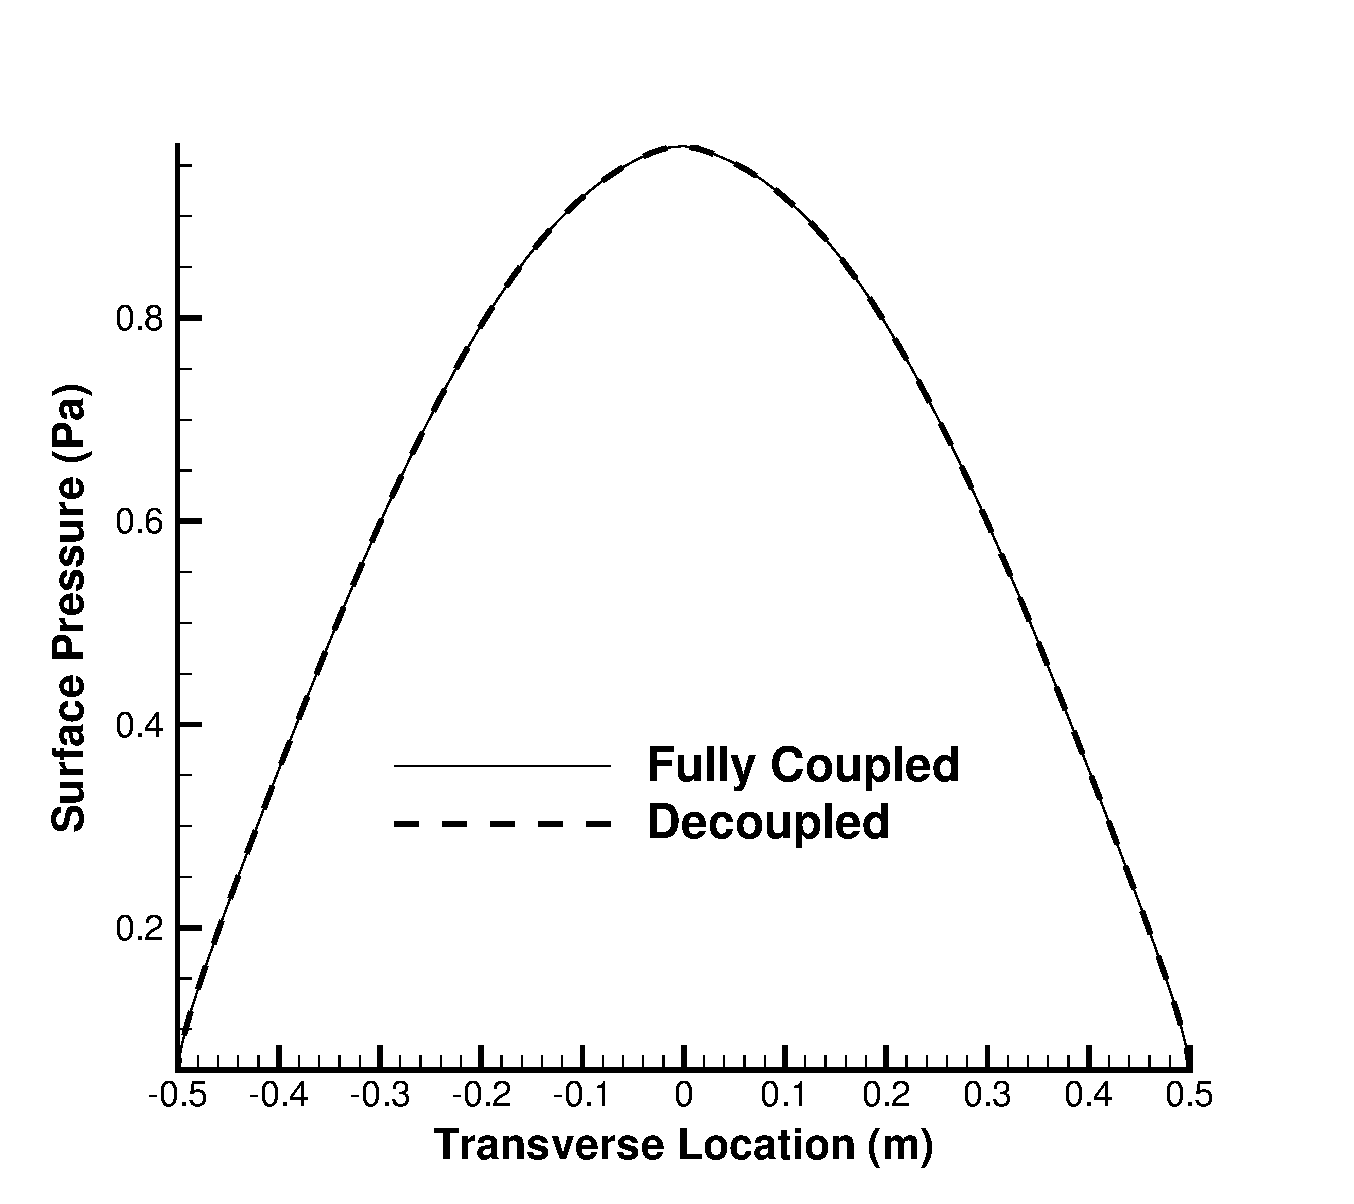
\includegraphics[width=\textwidth,trim={0 0 0 2cm}]{figures/surface_pressure}
          \end{figure}
        \end{column}
        \begin{column}{0.33\textwidth}
          \begin{figure}[h!]
            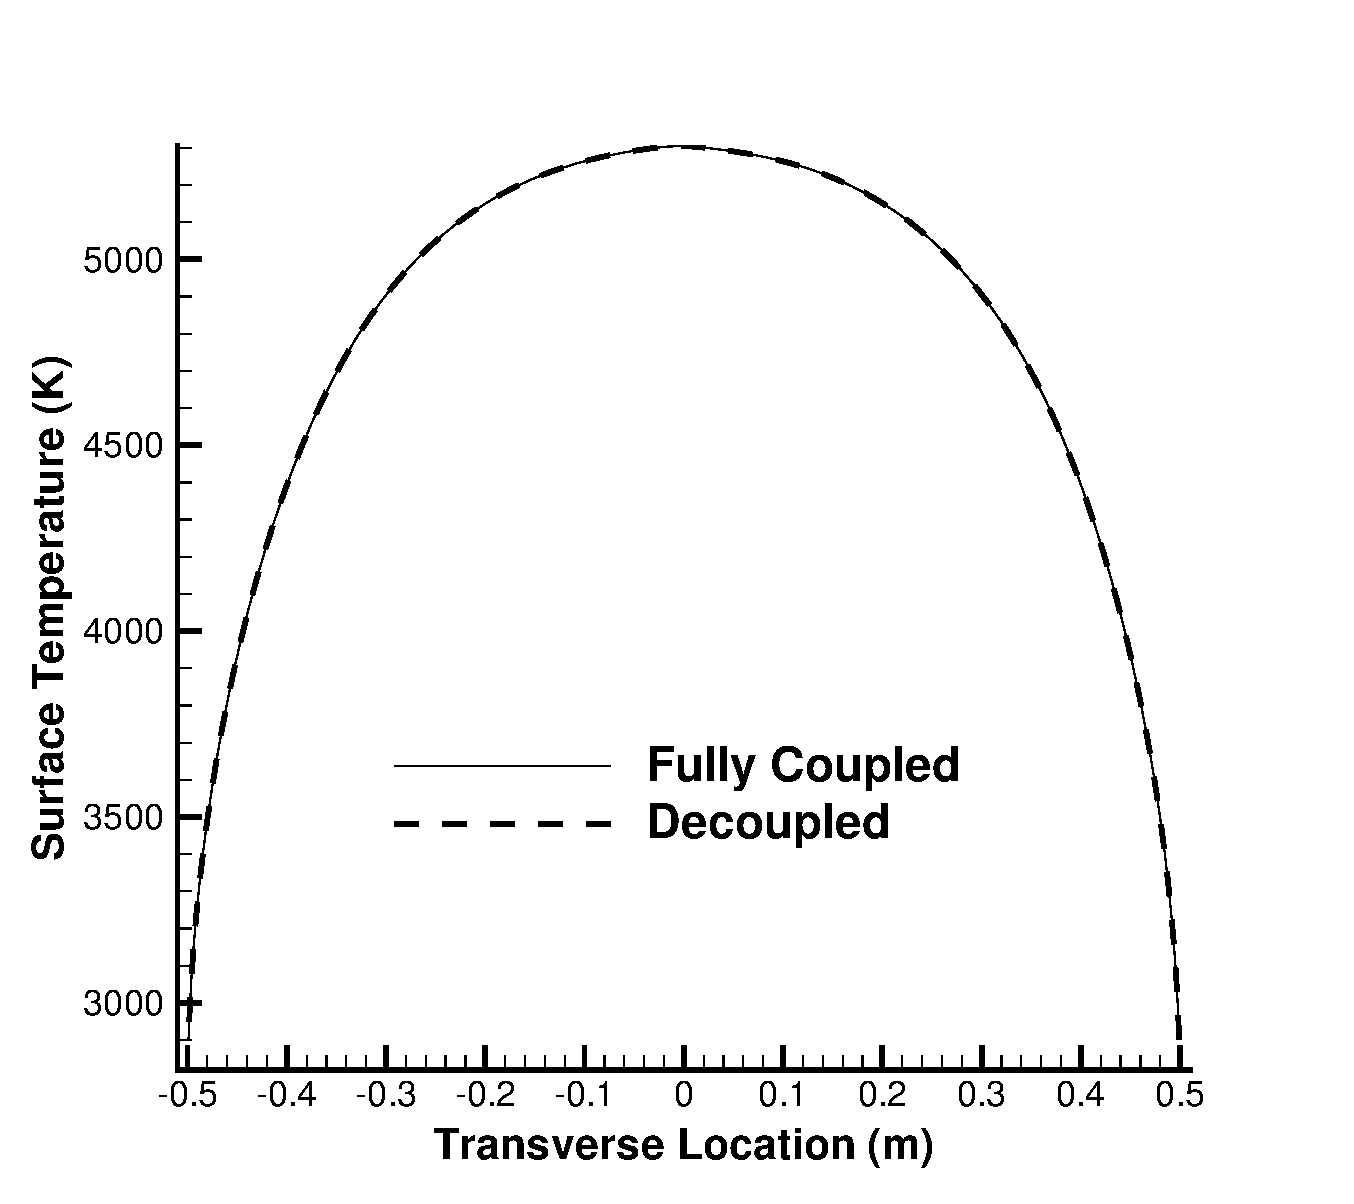
\includegraphics[width=\textwidth,trim={0 0 0 2cm}]{figures/surface_temperature}
          \end{figure}
        \end{column}
        \begin{column}{0.33\textwidth}
          \begin{figure}[h!]
            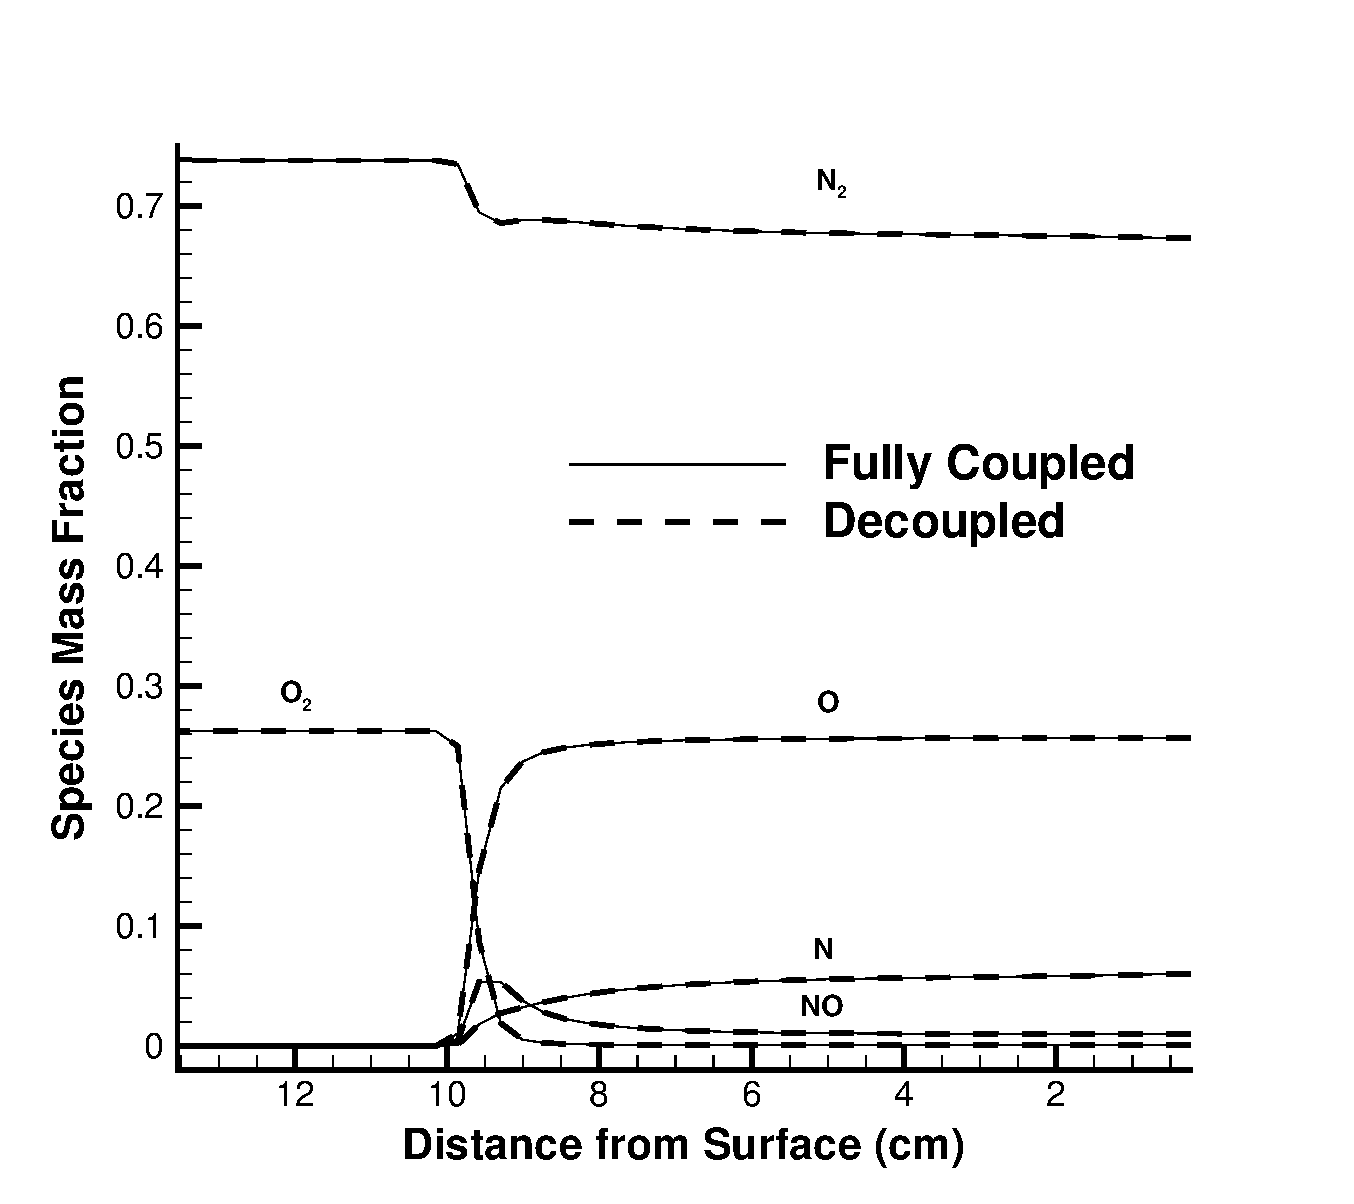
\includegraphics[width=\textwidth,trim={0 0 0 2cm}]{figures/stag_line_mf}
          \end{figure}
        \end{column}
      \end{columns}
      \vspace{3mm}
      \item Surface pressure and surface temperature agree discretely to 8 significant
        figures
      \item Mass fractions on stagnation line agree to 4 significant figures
    \end{itemize}
  \end{itemize}
\end{frame}
\begin{frame}
  \frametitle{Numerical Results: 2D Cylinder}
  \begin{columns}[t]
    \begin{column}{0.5\textwidth}
    \begin{figure}[h]
      \centering
      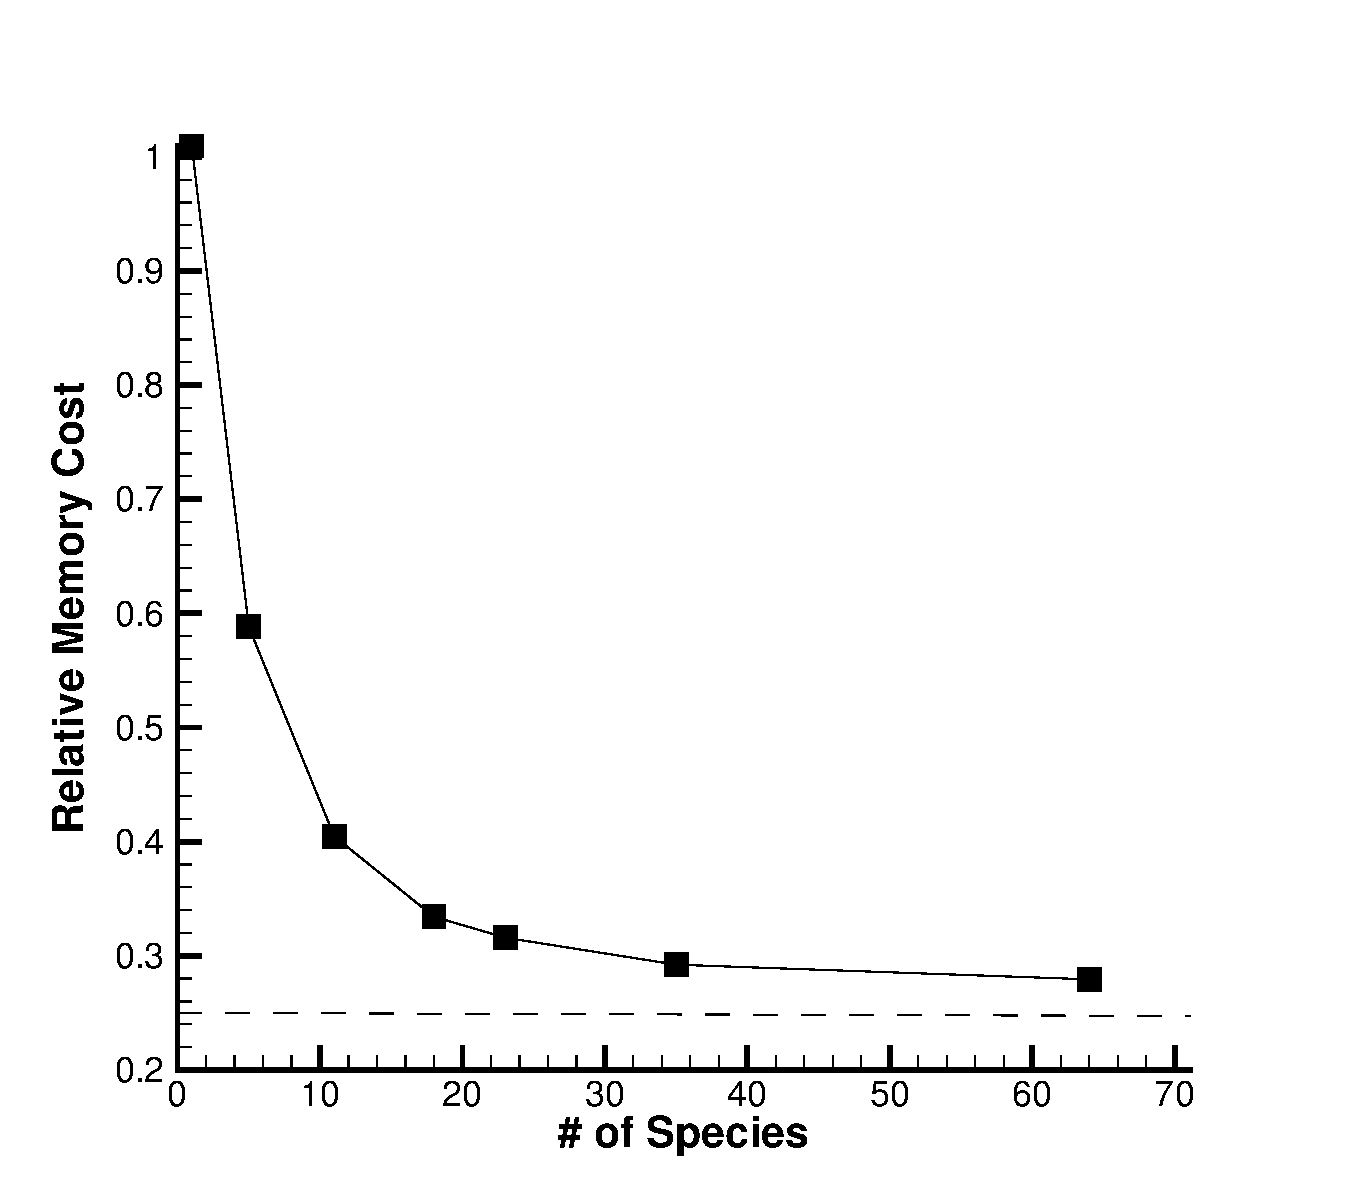
\includegraphics[width=0.8\textwidth,trim={0 0 1cm 2.5cm}]{figures/mem_req}
    \end{figure}
    \end{column}
    \begin{column}{0.5\textwidth}
      \begin{figure}[h]
        \centering
        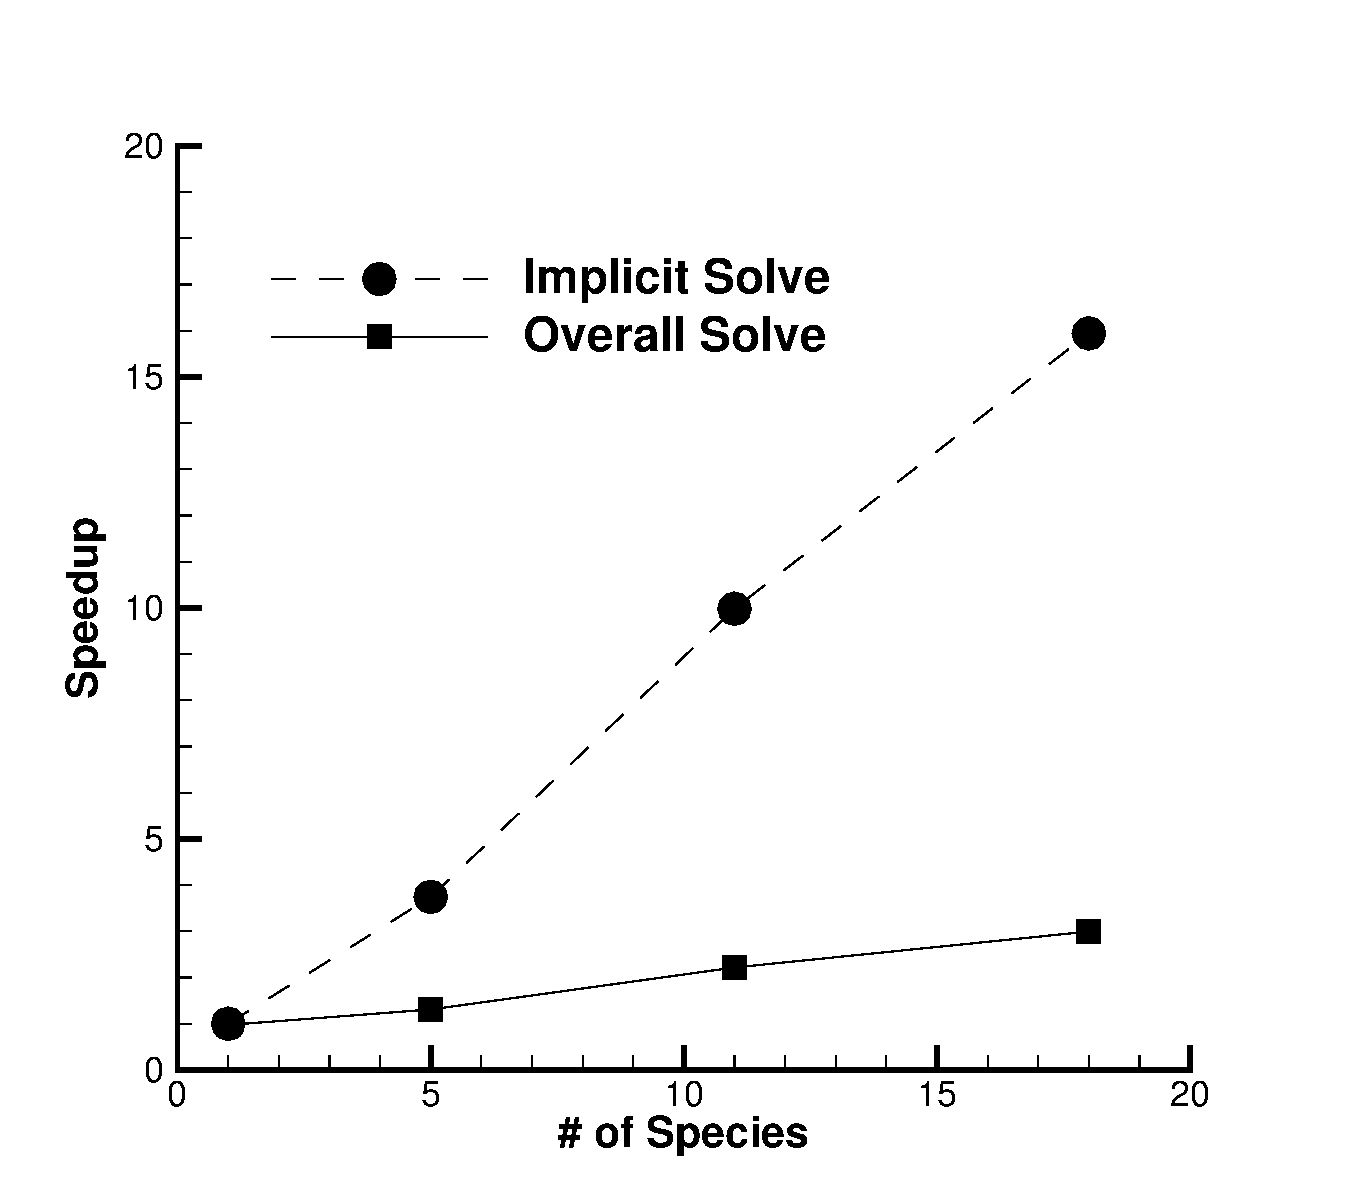
\includegraphics[width=0.8\textwidth,trim={1cm 0 0 2.5cm}]{figures/speedup} 
      \end{figure}
    \end{column}
  \end{columns}
  \begin{itemize}
    \item On structured grids $N_{nbrs} \approx 6 N_{nodes}$
    \begin{itemize}
      \item Half precision off-diagonal $N_{nbrs} = \frac{6N_{nodes}}{2}$
        \[ 
          Memory\ Cost \approx 
           \frac{N_{nodes}}{N_{nodes} + N_{nbrs}} =
           \frac{N_{nodes}}{N_{nodes} + 6N_{nodes}/2} = \frac{1}{4}
        \]
      \item Linear speedup in solver: $\frac{O(N^2)}{O(N)} = O(N)$
    \end{itemize}
  \end{itemize}
\end{frame}

\subsection{Axisymmetric Spherically Capped Cone}

\begin{frame}
  \frametitle{Numerical Results: Axisymmetric Spherically Capped Cone}
  \begin{figure}[h]
  	\centering
   \adjincludegraphics[width=0.7\textwidth,trim={0 3.5cm 0 3cm},clip]{figures/cone_mesh}
  \end{figure}
  \begin{itemize}
    \item Verify that the decoupled scheme is robust at high velocities
    \begin{itemize}
      \item $V_{\infty} = 15000\ m/s$, 
	$\rho_{\infty}=0.001\ kg/m^3$, $T_\infty = 200\ K$.
      \item 11-species air model N, $\text{N}_2$, O,
      $\text{O}_2$, NO, N$^+$, $\text{N}_2^+$, O$^+$, 
      $\text{O}_2^+$, NO$^+$, and electrons, with 22 possible reactions.
    \end{itemize}
  \end{itemize}
\end{frame}
\begin{frame}
  \frametitle{Numerical Results: Axisymmetric Spherically Capped Cone}
    \begin{columns}[t]
      \begin{column}{0.5\textwidth}
        \begin{figure}[h!]
          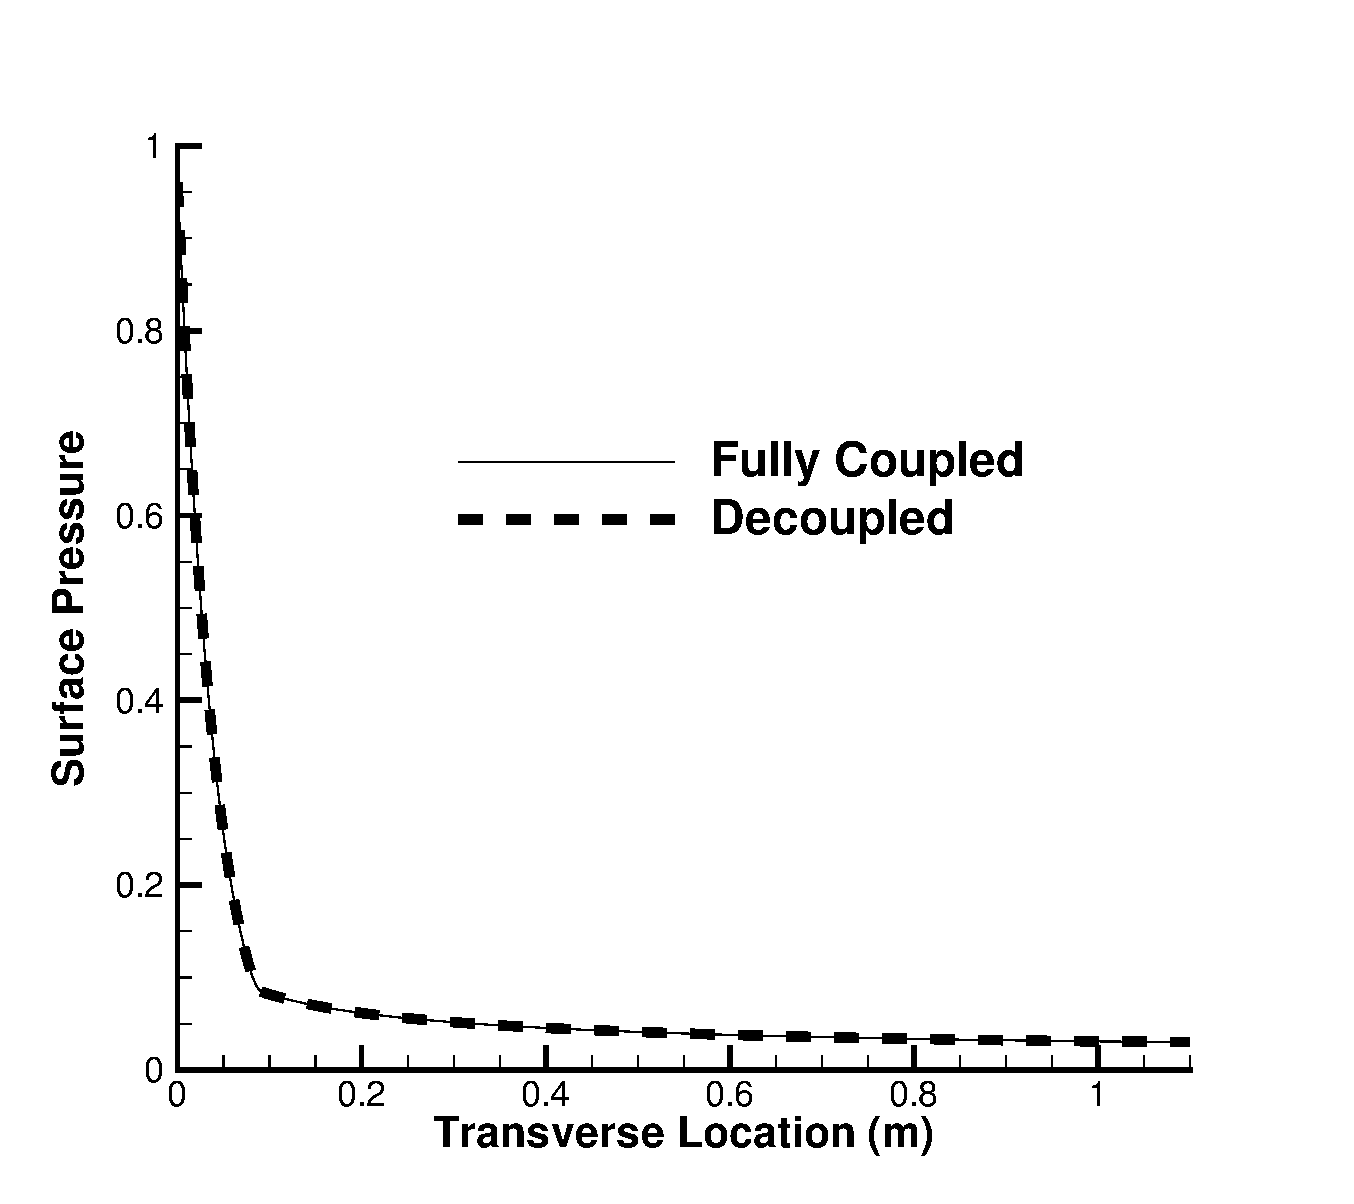
\includegraphics[width=\textwidth]{figures/surface_pressure_cone}
        \end{figure}
      \end{column}
      \begin{column}{0.5\textwidth}
        \begin{figure}[h!]
          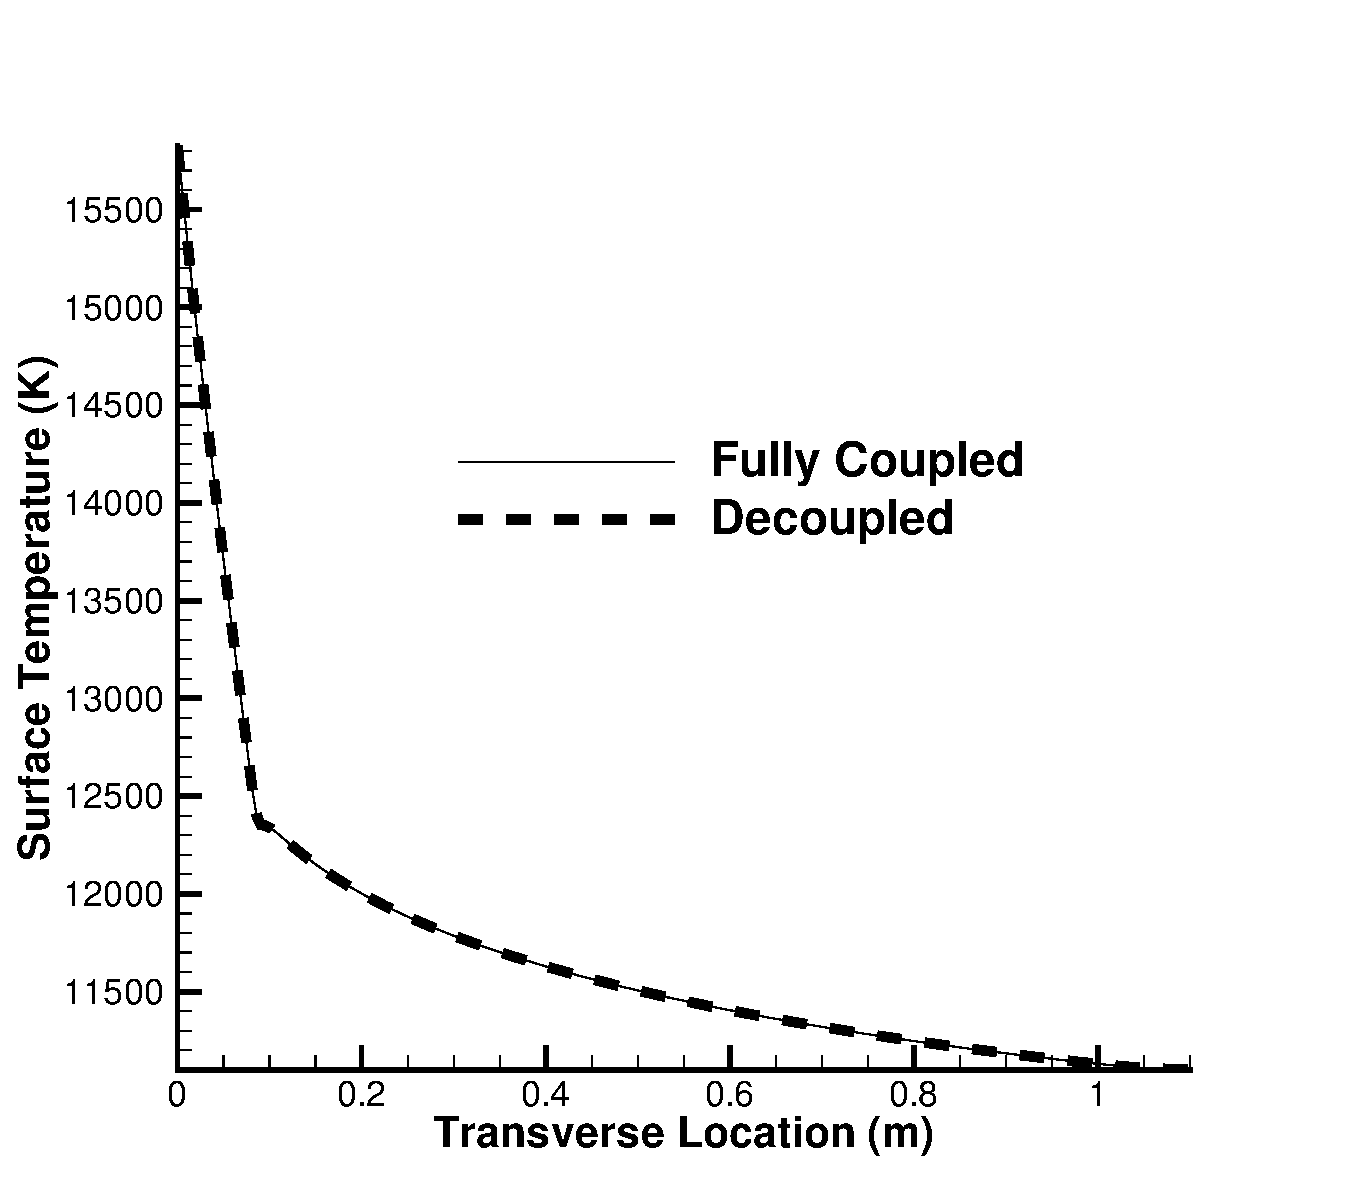
\includegraphics[width=\textwidth]{figures/surface_temperature_cone}
        \end{figure}
      \end{column}
    \end{columns}
    \begin{itemize}
      \item Surface pressure and surface temperature agree discretely 
	to 8 significant figures
    \end{itemize}
\end{frame}
\begin{frame}
  \frametitle{Numerical Results: Axisymmetric Spherically Capped Cone}
    \begin{columns}[t]
      \begin{column}{0.5\textwidth}
        \begin{figure}[h!]
    	  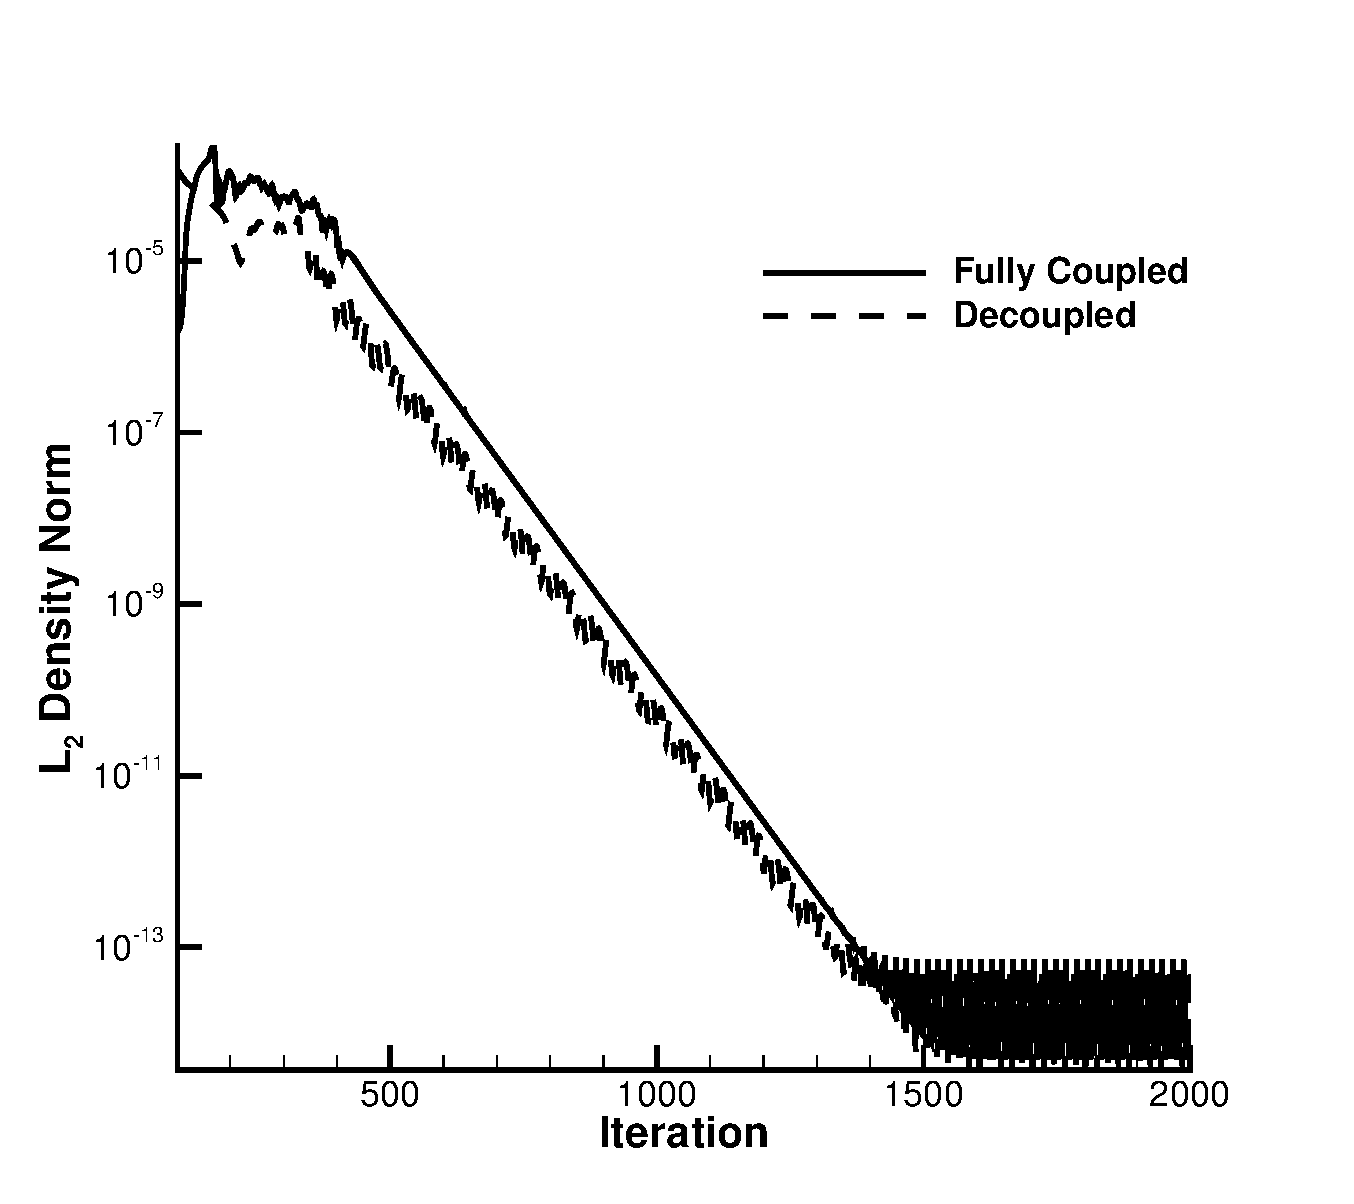
\includegraphics[width=\textwidth]{figures/cone_iteration}
        \end{figure}
      \end{column}
      \begin{column}{0.5\textwidth}
        \begin{figure}[h!]
	  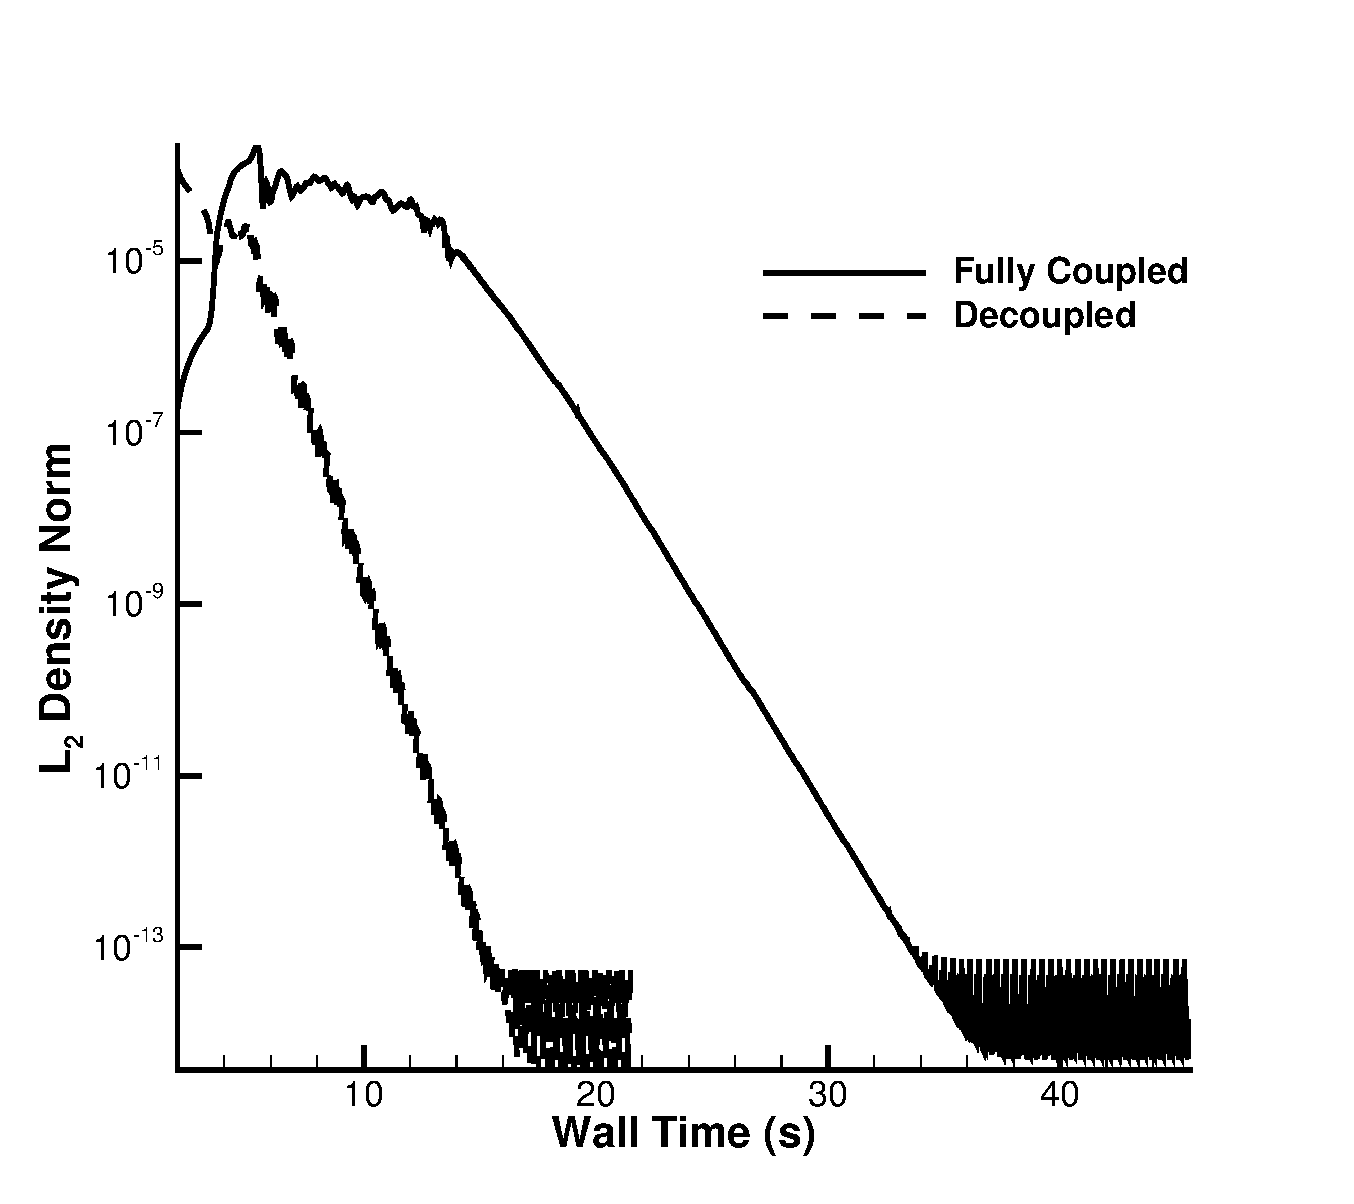
\includegraphics[width=\textwidth]{figures/cone_walltime}
        \end{figure}
      \end{column}
    \end{columns}
  \begin{itemize}
    \item Necessary to scale source term magnitude by $0.001 \leq w \leq 1$ 
      for the first 500 iterations, due to extreme reaction rates
    \item Both schemes converge in a similar number of iterations
    \item Decoupled scheme $\approx$ 2x faster
  \end{itemize}
\end{frame}

\section{Conclusions}
\stepcounter{subsection}

\begin{frame}
  \frametitle{Conclusions}
  \begin{itemize}
    \item Decoupling the species equations yield impressive benefits at minimal cost in robustness
      \begin{itemize}
        \item 2 times faster and 1/3 required memory for both 2D Cylinder and
          Sphere-Cone 11-species cases
        \item Convergence issues at very high velocities can be offset by
          scaling source term as solution progresses
      \end{itemize}
      \item Improvements valuable for adjoint work
        \begin{itemize}
          \item Preliminary testing has shown that memory overhead in adjoint is
            significantly reduced with decoupled scheme
          \item Can expect similar speedup in adjoint solve
          \item Differences between fully-coupled and decoupled method results
            may impact adjoint and require further study
        \end{itemize}
  \end{itemize}
\end{frame}
\begin{frame}
  \frametitle{Acknowledgements}
  \begin{itemize}
    \item The authors would like to recognize the FUN3D team at NASA
     Langley Research Center, for their support in integrating aspects of the
     compressible gas path into the reacting gas path of FUN3D.
   \item Thanks to the Entry Systems Modeling Project within the NASA
     Game Changing Development Program for their funding and support of this research.  
  \end{itemize}
\end{frame}

\section*{Backup}
\begin{frame}
  \frametitle{Backup: Derivation}
  \begin{itemize}
    \item For the Roe flux difference splitting scheme, the species mass fluxes are given by
  \[
  	F_{\rho_s} = \frac{\rho_s^L{\mU}^L+\rho_s^R{\mU}^R}{2}
  	-\frac{\tilde{c}_s(\lambda_1 dv_1 + \lambda_2 dv_2)+\lambda_3 dv_{3_s}}{2}
  \]
  \begin{align*}	
  		dv_1 &= \frac{p^R-p^L+\tilde{\rho} \tilde{a}
      ({\mU}^R-{\mU}^L)}{\tilde{a}^2} \\
  		dv_2 &= \frac{p^R-p^L-\tilde{\rho} \tilde{a}
      ({\mU}^R-{\mU}^L)}{\tilde{a}^2} \\
  		dv_{3_s} &= \frac{\tilde{a}^2 (\rho_s^R-\rho_s^L)- \tilde{c}_s (p^R-p^L)}{\tilde{a}^2}
  \end{align*}
  \begin{align*}
  	\lambda_1 = \mid \tilde{\mU}+\tilde{a} \mid,\quad 
  	\lambda_2 = \mid \tilde{\mU}-\tilde{a} \mid,\quad 
  	\lambda_3 = \mid \tilde{\mU} \mid
  \end{align*}
  \end{itemize}
\end{frame}
\begin{frame}
  \frametitle{Backup: Derivation}
  \begin{itemize}
    \item The $\tilde{}$ notation signifies a Roe-averaged quantity
    \begin{gather*}
    	\tilde{{\mU}} =w{U}^L+(1-w){\mU}^R \\
    	w = \frac{\tilde{\rho}}{\tilde{\rho}+\rho^R} \\
    	\tilde{\rho} = \sqrt{\rho^R\rho^L}
    \end{gather*}
    \item The species mass fluxes must sum to the total mass flux
    \[ F_\rho = \sum\limits_{s}{F_{\rho_s}} =
      \frac{\rho^L{\mU}^L+\rho^R{\mU}^R}{2}
    	-\frac{\tilde{c}_s(\lambda_1 dv_1 + \lambda_2 dv_2)+\lambda_3 dv_3}{2} \]
    \[ dv_3 = \frac{\tilde{a}^2 (\rho^R-\rho^L)-(p^R-p^L)}{\tilde{a}^2} \]
  \end{itemize}
\end{frame}
\begin{frame}
  \frametitle{Backup: Derivation}
  \begin{itemize}
    \item Substituting back into species mass flux equation
    \[
      F_{\rho_s} =\tilde{c}_s F_\rho +
      \frac{(c_s^L-\tilde{c}_s)\rho^L({\mU}^L+\mid \tilde{\mU}\mid)}{2} +
      \frac{(c_s^R-\tilde{c}_s)\rho^R({\mU}^R-\mid \tilde{\mU}\mid)}{2}
    \]
  \item This can be simplified to yield a form similar to that derived by
    Candler, et. al for the Steger-Warming scheme
  \[
    F_{\rho_s} =\tilde{c}_s F_\rho +
    (c_s^L-\tilde{c}_s)\rho^L\lambda^+ + (c_s^R-\tilde{c}_s)\rho^R\lambda^-
  \]
  \[
    \lambda^+ = \frac{{\mU}^L+\mid
    \tilde{\mU}\mid}{2}, \quad \lambda^- = \frac{{\mU}^R-\mid
    \tilde{\mU}\mid}{2}
  \]
  \end{itemize}
\end{frame}
\begin{frame}
  \frametitle{Backup: Derivation}
  \begin{itemize}
    \item Differentiating with respect to the mass fraction, $c_s$, the left and
      right state contributions are
    \begin{align*} \frac{\partial F_{\rho_s}}{\partial c^L_s} &=
      wF_\rho+(1-w)\rho^L\lambda^+ - w\rho^R\lambda^- \\ 
      \frac{\partial F_{\rho_s}}{\partial c^R_s} &=
      (1-w)F_\rho+(w-1)\rho^L\lambda^+ + w\rho^R\lambda^- 
    \end{align*}
  \item Again, where $w$ is the Roe-averaged density weighting
    \[
    	w = \frac{\tilde{\rho}}{\tilde{\rho}+\rho^R},\quad
    	\tilde{\rho} = \sqrt{\rho^R\rho^L}
    \]
  \end{itemize}
\end{frame}

\end{document}

